\documentclass[12pt]{article}
\usepackage{geometry}
\geometry{a4paper}
\usepackage[round]{natbib}
\usepackage{graphicx}
\usepackage[T1]{fontenc}
\usepackage[utf8]{inputenc}
\usepackage{textcomp}
\usepackage{gensymb}
\usepackage{amsmath}
\usepackage{amssymb}
\usepackage{authblk}
\usepackage[running]{lineno}
\usepackage{setspace}
\usepackage{rotating}
\usepackage{hyperref}

\setlength{\parindent}{0pt}


\usepackage{fancyhdr}
 
\pagestyle{fancy}
\fancyhf{}
\rhead{Tad Dallas (Biol 4253)}
\lhead{Macroecology}

\doublespacing




\begin{document}










\subsection*{Reading:}

McGill, Brian J. "The what, how and why of doing macroecology." Global Ecology and Biogeography 28.1 (2019): 6-17. \\ \url{https://onlinelibrary.wiley.com/doi/pdf/10.1111/geb.12855} \\

\bigskip

%Shade, A., Dunn, R. R., Blowes, S. A., Keil, P., Bohannan, B. J., Herrmann, M., ... \& Chase, J. (2018). Macroecology to unite all life, large and small. Trends in Ecology \& Evolution. \\ \url{https://www.indiana.edu/~microbes/publications/Shade_etal_2018_InPress.pdf} \\




\begin{center}
\noindent\hrulefill 
\end{center}



\clearpage



\subsection*{How do we scale small scale processes to global scales?}

The goal of the field of \textit{macroecology} is to explain variation in species abundance, distribution, and diversity, particularly over large geographic scales. It's useful to talk about at this stage in the semester because we've focused a lot on relatively local processes (e.g., competition in a single area). Many macroecological relationships do not have a clear mechanism, often ignore species differences, and almost exclusively do not consider many ecological processes we've discussed (e.g., competition, predation). Much of this relates to classic ecological theory on the importance of spatial scale. One idea is that some processes such as competition and predation are important largely important at very local (smaller) scales. As we "zoom out" to more coarser scales, the role of environment becomes more pronounced in determining species diversity and abundance. This is often referred to as the \textit{Eltonian noise hypothesis}. 









\paragraph*{The transmutation problem}

Sometimes spatial scale can determine whether a pattern is observed at all. That is, a series of relationships at more local scales that can be either positive or negative can result in a clear pattern at larger spatial scales. McGill 2019 goes into a lot of detail about \textit{transmutations}, which explore how different hierarchical scales may be entirely different. 


A simple example is in the scaling between a local to macro scale comparison of the relationship 
between precipitation and productivity. This is the idea that areas that receive more precipitation, on average, have higher productivity (more green biomass, essentially). But this is a bit site-specific, right? We can imagine that productivity could go up with precipitation if plants require more water, but the opposite relationship could be observed as nutrients are washed away from the soil and plants are exposed to too much water. While the local context would suggest no clear relationship, plotting a series of these local relationships yields a general macroecological relationship between precipitation and productivity. 




% \paragraph*{Jensen's inequality}






\paragraph*{}

Macroecological relationships allow scientists to undercover generalized \textit{laws} about how biodiversity is distributed. That is, at some spatial scale, the influence of many small scale ecological processes will become relatively unimportant, and global (or macro) scale patterns will emerge. We'll go over some examples of macroecological laws here, and be sure to read to the McGill paper for more information on the historical and conceptual history of macroecology.
 







\paragraph*{The dimensionality of macroecology}

The scope of macroecology is perhaps best depicted in terms of spatial, temporal, and taxonomic scales of study. How many of these do you think would need to be incorporated to qualify as "macroecology"?

\begin{figure}
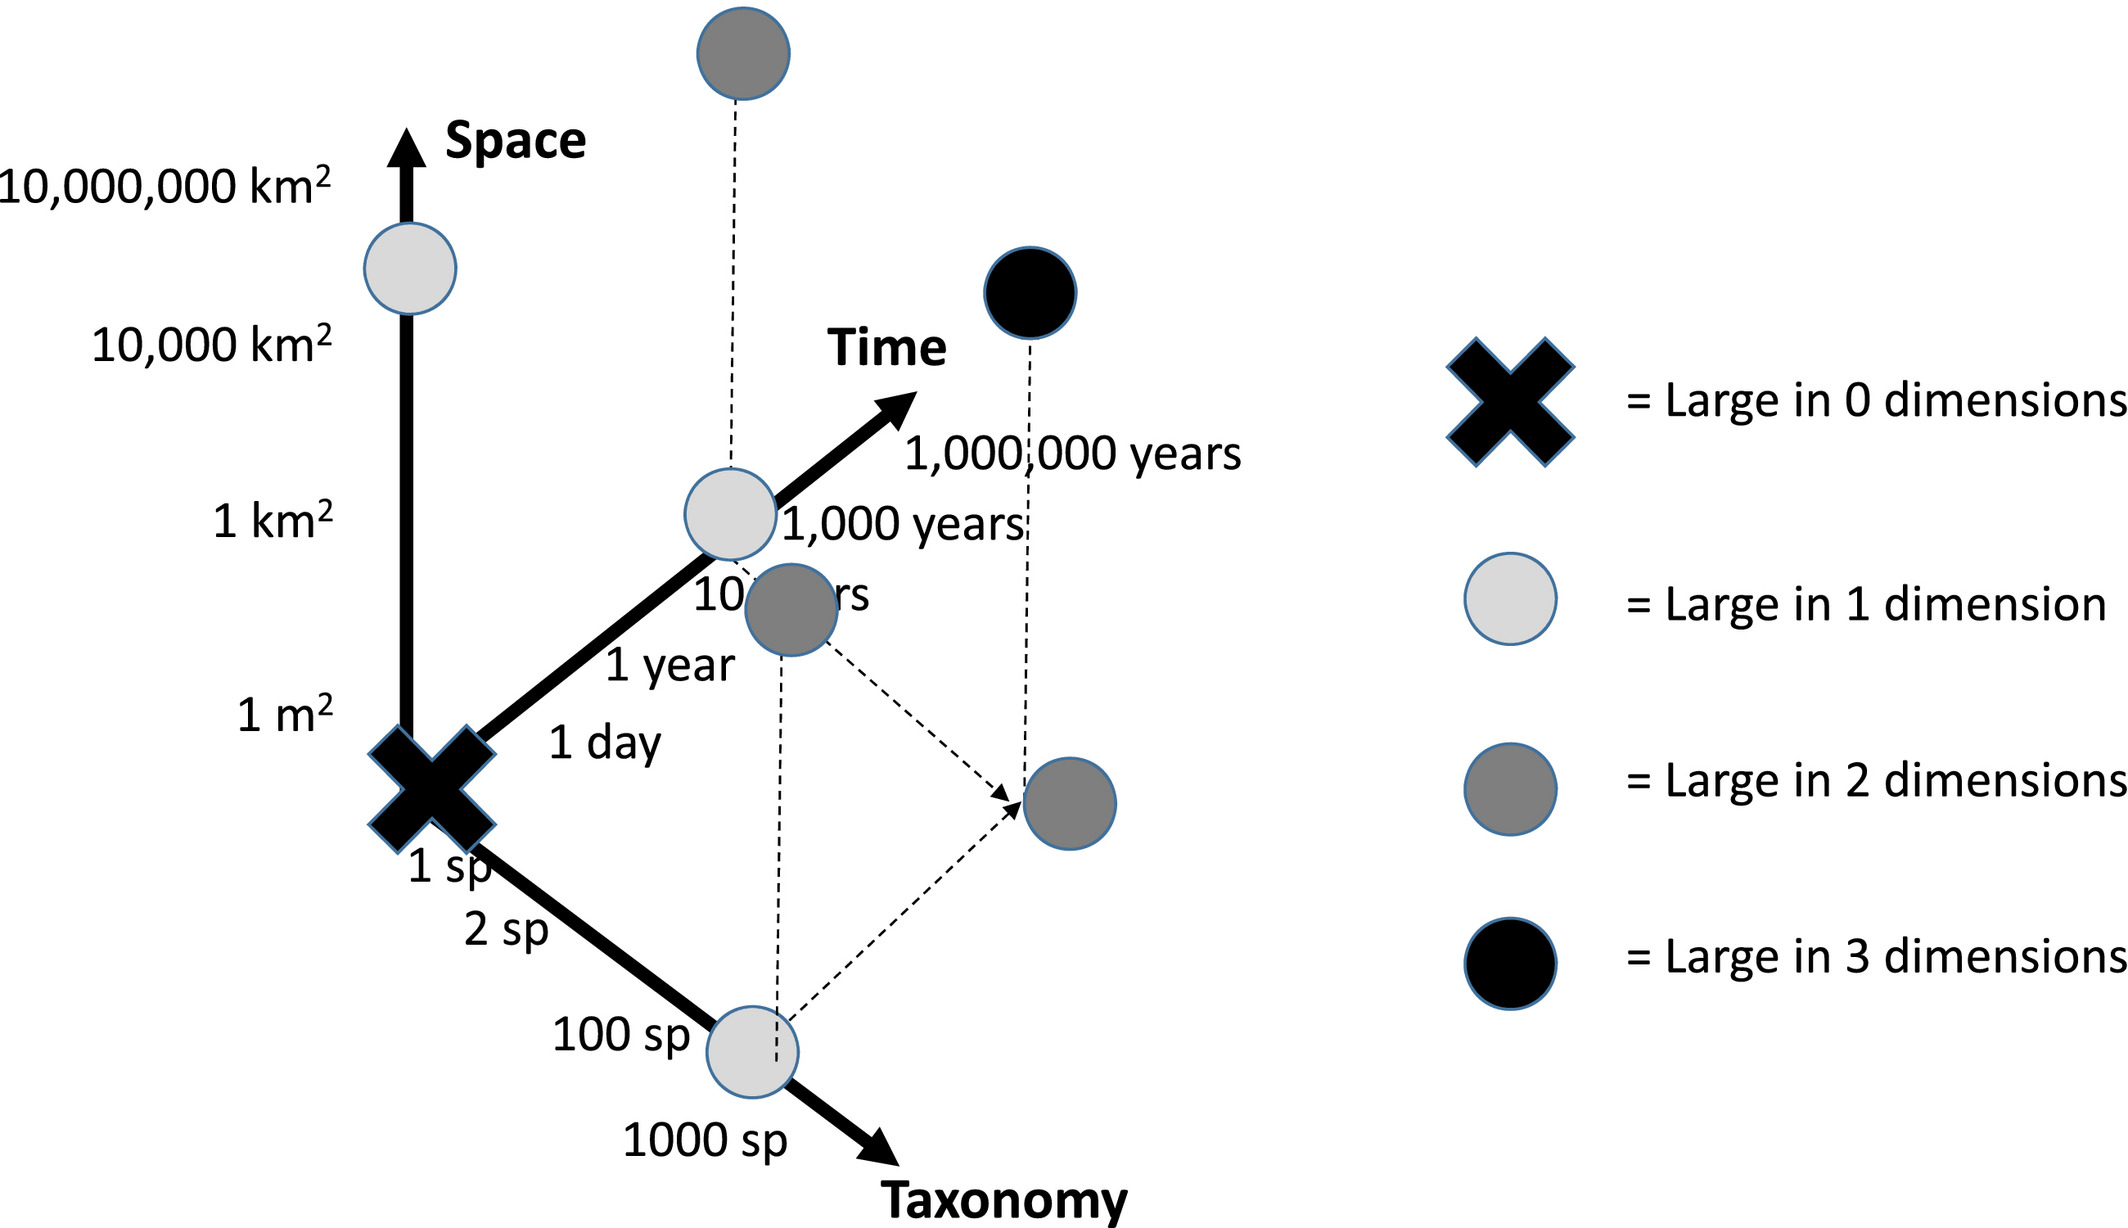
\includegraphics[width=\textwidth]{figs/macro.jpg}
\caption{Figure taken from McGill (2019) https://doi.org/10.1111/geb.12855.}
\end{figure}
















\bigskip

\subsection*{Latitudinal scaling}

Latitude is a major driver of variation in species diversity and range dynamics. Latitudinal variation represents large climatic variation, but could also relate to solar radiation, historical biogeographic processes, land area, etc.



\bigskip




\paragraph*{Latitudinal diversity gradient}

Species richness (alpha diversity) tends to be highest near the equator, and declines toward the poles. This pattern has been studied for many different groups of organisms (including parasites!) and is pretty consistent. As with many macroecological patterns though, it is difficult to attribute mechanism to the pattern. Latitude is not really an ecologically driver, but temperature, precipitation, land area, and geological history are all associated with latitude in some form. 

\textit{species-energy hypothesis}: the amount of energy sets limits to the species richness an area can achieve (relate this back to food web structure). So more primary productivity in lower latitudes through increased light availability leads to more species in the food web.  \\

\textit{climatic stability hypothesis}: Fluctuating environments tend to cause species extinctions. Environmental conditions tend to fluctuate more at higher latitudes. \\


\textbf{The mid-domain effect}

The inherent constraints on latitude and shifting species ranges causes species richness to peak at middle latitudes. That is, assuming the random placement of a species with some fixed latitudinal range, there will still be more species near the equator. \\




((draw this out)) \\






The mid-domain effect doesn't mean that we shouldn't look for latitudinal diversity relationships, but we should recognize that they could be the result of randomness. Teasing the randomness from the pattern sometimes requires the use of a \textit{null model}. In the case of the mid-domain effect, a null model would correspond to shuffling species ranges around and measuring the strength and variation in the resulting latitudinal diversity relationship. We also talked about null models a bit when we discussed ecological networks (specifically the importance of a single node to a property of the entire network). 







\bigskip















\paragraph*{Rapoport's rule}

Latitudinal variation can also be observed species range sizes. Rapoport's rule argues that the latitudinal ranges (minimum latitude to maximum latitude where a species is found) of species tend to be smaller near the equator. This is actually one of the potential reasons for the latitudinal diversity gradient as well. Smaller latitudinal ranges means that you can pack more species into a given area without so much species overlap, resulting in higher diversity near the equator as a function of smaller latitudinal ranges.

















\bigskip




\paragraph*{Bergmann's rule}

A final latitudinal scaling rule we'll talk about is the scaling of species body sizes with latitude. Bergmann's rule argues that the average body mass of species increases moving away from the equator (so species body size is smallest at the equator and largest near the poles). The support for this comes in the form of two different ways to examine this. \\

First, the rule can be examined within a single species across its latitudinal range. This is perhaps the clearest support for the relationship. \\

Second, the rule can be examined considering all species in a given area, where the mean body size for all organisms within the same trophic level or taxa is tracked across latitude.\\

These two approaches tend to yield the same results, and oftentimes it's really tough to get data to address the first way, but fairly straightforward to get data to test the second. 






















\bigskip



\subsection*{Species abundance distributions}

Species abundance distributions are common ways to describe the structure of ecological communities, and can be compared across spatial gradients. For a given area, the species abundance distribution is really similar to the rank abundance distribution, which we went over previously. Here, the x-axis is species counts (abundances) and the y-axis is the frequency that a species is found with that abundance (so the number of species which fall into a given abundance class). The shape of the relationship is important, because different proposed mechanisms will lead to different shapes. We won't go over the details about the different models for explaining the shape of the species abundance distribution, but you should know that pretty much every ecological community species abundance distribution has a \textit{hollow curve} shape with many rare species and just a few common species. 







\bigskip




\paragraph*{Abundant-center hypothesis}

The abundant center hypothesis is a classic distance-abundance relationship, where we relate some measure of distance of a population to an aspect of the species entire range to species abundance at that particular site. Specifically, the abundant center hypothesis states that species density should be highest in the center of species range. \\



((sketch this in notes to clarify)) \\


This makes a number of assumptions, some of which are:

\begin{itemize}
  \item species densities represent equilibrial populations across space
  \item species interactions (predation, parasitism, etc.) do not influence species density
  \item geographic center of a range also corresponds to the center of the niche?
\end{itemize}


So how do we operationalize this relationship? We measure species density across a species range, we calculate the range boundaries and measure distance (either to the range center or to the range boundary) and then we regress species density (y-axis) and the measure of distance we went with. If we measured distance from the range edge, we would expect a negative relationship between distance and abundance (density) if distance was measured as distance from the range center, and a positive relationship if distance was measured as distance from the range edge. 











\bigskip
\subsection*{Conclusions}
















\end{document}
